\documentclass[a4paper,12pt,report]{jsbook}

%ページに綴じ代をつくる
\setlength{\textwidth}{38zw}
\setlength{\oddsidemargin}{0.5cm}


%共通設定
\renewcommand{\bibname}{参考文献}
\renewcommand{\theenumi}{\roman{enumi}}
\usepackage{makeidx}
\pagestyle{headings}
\usepackage[dvipdfmx]{graphicx}
\pagenumbering{roman}
\usepackage{bm}
\usepackage{multirow}
\usepackage{amsmath}
\usepackage{amssymb}
\usepackage{amsfonts}
\usepackage{mathtools}
%\usepackage{math}



%枠関連の設定
\usepackage{fancybox}
\usepackage{framed}
\newenvironment{longbox}{%
  \def\FrameCommand{\fboxsep=\FrameSep \fbox}%
  \MakeFramed {\FrameRestore}}%
 {\endMakeFramed}

\makeindex

\begin{document}



%
% 表紙
%
\begin{titlepage}
\begin{center}
{\large 令和04度卒業論文\\}
\vspace{2.5cm}
{\fontsize{36pt}{40pt}\selectfont%
 自己注意による\\
 コンテクスト抽出を\\用いた\\画像ノイズ除去手法\\}
\vspace{3cm}
{\large%
  千葉工業大学 先進工学部 \\
  \vspace{3mm}19C3020 有働 和矢\\
  \vspace{3cm}指導教員 宮田 高道 教授\\
  \vspace{1cm}提出日 令和2023年1月17日\\
}%各所にあるvspaceの値を調整して1ページに収まるようにしましょう.
\end{center}
\end{titlepage}

%%%%%%%%%%%%%%%%%%%%%%%%%%和文要旨%%%%%%%%%%%%%%%%%%%%%%%%%%%%%%
\begin{titlepage}
\begin{longbox}
\begin{center}
 {\Huge 自己注意によるコンテクスト抽出を用いた画像ノイズ除去手法\\}
 {\large%
   \vspace{3mm}%
   19C03020 有働 和矢\\
 }
\end{center}
{\bf 概要:}%
Transfomerに代表される自己注意機構を利用することが画像処理の分野で拡がっている. 画像ノイズ除去タスクにおいて長距離間の依存関係を認識できる自己注意機構を応用することにより, 画像のコンテクストを把握しながらノイズ除去を行うことが可能となるため, 高いノイズ除去性能が実現できることが明らかになっている. 一方でコンテクスト抽出と(抽出したコンテクストに基づく)ノイズ除去の二つのタスクを異なる二種類のCNNで行うことで効率的にノイズ除去を行えるGTCNNと呼ばれる手法が提案されており, 画像ノイズ除去タスクにおいてコンテクストの把握とノイズ除去処理のすべてを自己注意機構のみで行うことはCNNと同様に効率的でない可能性がある. そこで本研究ではGTCNNのコンテクストを抽出するCNNを自己注意に置き換えたSAGTCNNを提案する. 実験結果より, GTCNNと比較して高いノイズ除去性能またはより効率的なノイズ除去性能を得ることは叶わなかった. 本実験では画像サイズの小さい領域でしか自己注意を用いなかったり, ViT等の画像処理に自己注意を活用する手法で行われている位置埋め込みを行なっていないなどの理由から自己注意が本来の性能を発揮できなかった可能性が考えられる.
\\
\\
\end{longbox}
\end{titlepage}
%%%%%%%%%%%%%%%%%%%%%%%%%%%%%%%%%%%%%%%%%%%%%%%%%%%%%%%%%%%%%%%%

%%%%%%%%%%%%%%%%%%%%%%%%%%%%%%%%%%%%%%%%%%%%%%%%%%%%%%%%%%%%%%%%


\bibliographystyle{junsrt}
%\maketitle
\setcounter{tocdepth}{3}
\tableofcontents


\newpage
\pagenumbering{arabic}
\setcounter{page}{1}

%%%%%%%%%%%%%%%%%%%%%%%ここから本文を書きましょう%%%%%%%%%%%%%%%
%各章毎にファイルを分割して\inputで読み込ませると管理が楽
\chapter{序論}
\section{背景}
画像ノイズ除去はノイズが発生した画像から, ノイズを含まない原画像を推定することを目的としており, 画像処理分野における基礎的なタスクであることから多様な研究が行われている. 
近年, 自動運転や監視カメラ, 医療などの分野において画像認識技術が幅広く活用されており, 今後もその対象は拡がっていくと予想されている前述の画像ノイズ除去は, このような画像認識の認識精度を向上させるための前処理としても重要な役割を担っている.\\
 現在, 画像のノイズ除去においては高いノイズ除去性能を持つ深層学習を用いた手法が主流となっており, 特に深層畳み込みニューラルネットワーク(CNN)が高い性能を示すことが明らかになっている. CNNの欠点としては, 畳み込み層の受容野が比較的狭く,長距離の画素間依存性を認識できないことが挙げられる. このため, 既存のCNNを用いた画像のノイズ除去手法では, 画像の持つコンテクスト(文脈情報)を判断することが困難であり, 除去すべきノイズと残すべき細部の特徴とを区別できないことが知られている.\\
 このようなCNNの問題を解決するための新たな手法として, Transfomer\cite{SA}に代表される自己注意機構を利用することが画像処理の分野で拡がっている\cite{ViT,Swin}. 自己注意機構は自然言語処理の分野で開発された手法で, 離れた位置に存在する単語間の関係を認識することで, 様々な自然言語処理を高精度で行えることが明らかになっている. 長距離間の依存関係を認識できる自己注意機構をノイズ除去に応用することにより, 画像のコンテクストを把握しながらノイズ除去を行うことが可能となり, 高いノイズ除去性能が実現できることが明らかになっている\cite{Swin,Restormer}. 一方で, コンテクスト抽出と(抽出したコンテクストに基づく)ノイズ除去の二つのタスクを異なる二種類のCNNで行うことで効率的にノイズ除去を行えるGTCNNと呼ばれる手法が提案されており\cite{GTCNN}, 画像ノイズ除去タスクにおいてコンテクストの把握とノイズ除去処理のすべてを自己注意機構のみで行うことは, CNNと同様に効率的でない可能性がある.

\section{目的}
前述のようにノイズ除去の二つのタスクを異なる二種類のCNNで行うことで効率的にノイズ除去を行うことができる. このうちコンテクスト抽出タスクを行うCNNをCNNよりコンテクスト把握に有効であるといわれている自己注意機構に置き換えることで, 既存手法と比較してより高いノイズ除去性能または効率的なノイズ除去性能を得ることを目的とする.
\chapter{関連研究}

\section{Gated context CNN}
Gated context CNN (以下GTCNN) は, 図\ref{fig:GTCNN_overall}に示すように入力層, 出力層, 中間層である$L$個のGCBR層(Gated CBR Layer)からなる. GCBR層はノイズ除去のみを行うCNN (CBR) とコンテクスト抽出のみを行うCNN (GTL) とに分離されている. GTLが抽出したコンテクストはgate機構を介してCBRに渡されノイズ除去を制御する. このように機能分離を行うことで, 機能分離を行わない既存手法と比較して高いノイズ除去性能を獲得でき, またパラメータ数の削減に成功した. 


\subsection{GTL}
GTLはマルチスケール構造のU-Net\cite{U-net}をベースに設計されている. 一般的なU-Netのエンコーダは$S$段の層を持ち, その階層が下がるたびに特徴量のスケールを半減させ, チャンネル数を倍増させる. デコーダはエンコーダと同数の$S$段の層を持ち, 階層が上がるたびに特徴量のスケールを倍増させ, チャンネル数を半減させる. エンコーダ側では段階的にスケールのサイズが半減するため, CNNのカーネルのサイズが一定でも受容野の広さが倍に増大し, これによって広くコンテクストを把握できるようになる. 一方で, チャンネル数を倍増させることが計算コストの増大にもつながる. GTLでは, 階層を下げるときにチャンネル数を増やさないように変更を加えることで計算効率を高めている. 一般的なU-Netを用いたノイズ除去とはことなり, GTCNNのGTLはコンテクストの把握のみに注力できる(ノイズ除去はCBR層が行っている)ため, チャンネル数を増加させずとも良い性能が得られていると推測されている. 


\begin{figure}[ht]
\centering
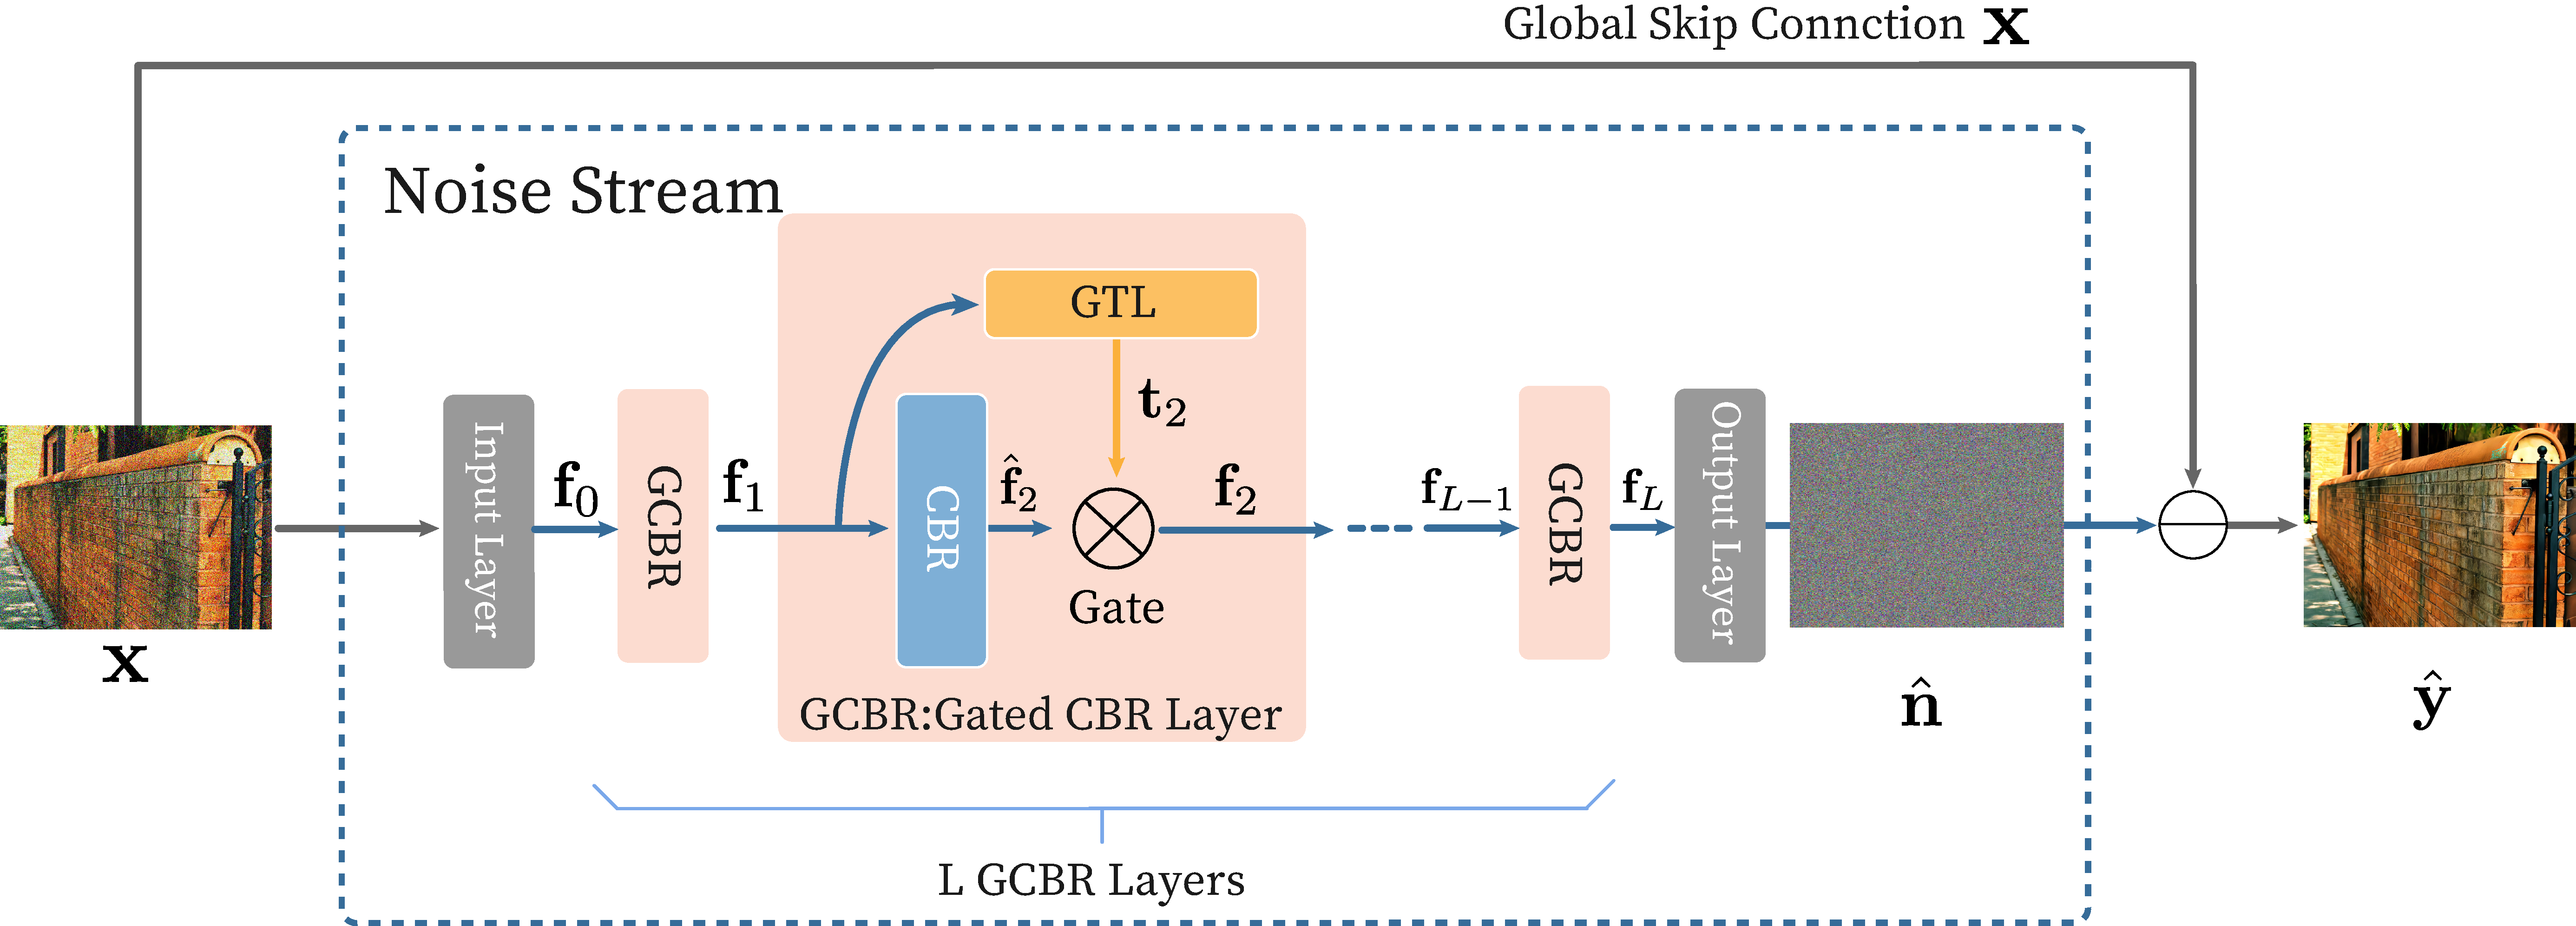
\includegraphics[scale=0.13]{figures/GTCNN_overall.pdf}
\caption{GTCNNのアーキテクチャ全体図. 文献\cite{GTCNN}より引用. (C) 2020 Springer \label{fig:GTCNN_overall}}
\end{figure}

\section{Vition Transformer}
Vision Transformer (ViT) \cite{ViT}は自然言語処理の分野で用いられていたTransformerを画像処理の分野で活用可能なものにし, また画像分類タスクの性能を向上をさせた手法である. それまで画像処理タスクはCNNに大きく依存しており, またCNNはその性質上広域なコンテクストの取得が難しかった.\\
 ViTは画像を複数のパッチの集合とすることで自己注意主体のネットワーク構造で画像を処理することが可能となった. パッチをトークンに見立て, それに一般的なTransformer同様に埋め込み処理を行いそれをTransformerのEncoderに入力する. そして出力されたデータをMLPを通しクラスデータを抽出する.\\
 図\ref{fig:vit_overall}のTransformer Encoder部を式で記述すると以下のようになる. Transformer Encoderにはパッチに埋め込み処理を施されたデータ$\bm{z}_{0}$が初めに入力される.
 \begin{align}
\bm{z}^{\prime}_{l} &= MSA(LN(\bm{z}_{l-1})) +\bm{z}_{l-1},& &l = 1 \cdots L \\
\bm{z}_l &= MLP(LN(\bm{z}^{\prime}_{l})) + \bm{z}^{\prime}_{l},& &l = 1 \cdots L
 \end{align}

$LN$はレイヤーノルム, $MLP$は多層パーセプトロン, $MSA$が自己注意を表している. 自己注意は式(\ref{eq:SA})のように表される\cite{SA}. $\mathbf{Q,K,V}$は入力にそれぞれ異なる埋め込み処理をしたものである.
\begin{align}
Attention(\mathbf Q,\;\mathbf K,\; \mathbf V)=softmax(\frac{\mathbf Q \mathbf K^T}{\sqrt{d_k}})\mathbf V \label{eq:SA}
\end{align}
 式(\ref{eq:SA})では$\mathbf{Q}$と$\mathbf{K}$から得られる全データ間の類似度をもとに, $\mathbf{V}$を処理することを表しており, このことから, 局所的な処理をするCNNとは異なり, 自己注意は大域的な処理を行っているということである. ViTではこの特性のため広域なコンテクストの取得を可能とした. しかし自己注意機構には, 入力データ長の二乗に比例し計算量が増えてしまう課題が存在する.

\begin{figure}[ht]
\centering
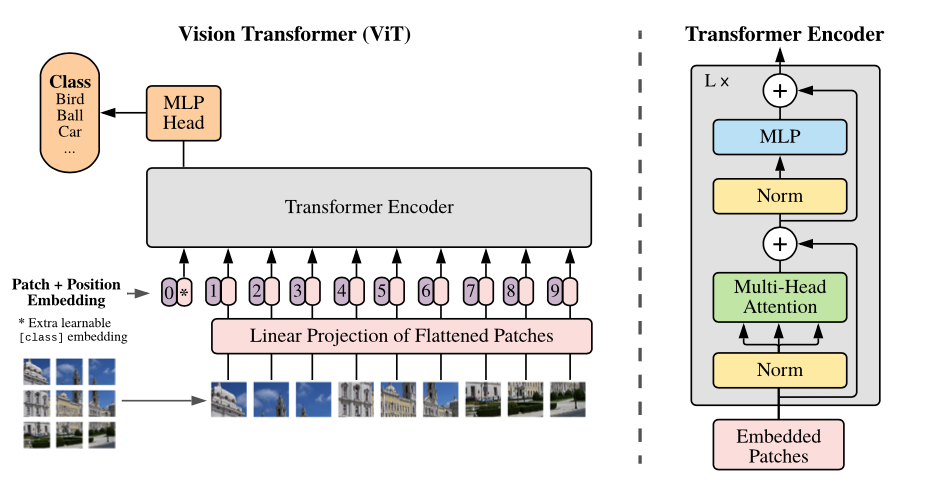
\includegraphics[scale=0.4]{figures/vit_overall.png}
\caption{ViTのアーキテクチャ全体図. 文献\cite{ViT}より引用. (C) 2021 ICLR \label{fig:vit_overall}}
\end{figure}

\newpage
\section{Restormer}
Restormer\cite{Restormer}はTransformerを活用した手法で, ノイズ除去をはじめとした画像復元タスクにおいて高い性能を示す. 図\ref{fig:Restomer_overall}の通りU-Netをベースに作られており, 各層にはTransformer Blockが配置されている. またTransfomer Blockの数は階層が下がるほど増加する. Transformer BlockにはMulti-Dconv head transposed attention (MDTA) とGated-Dconv feed-forward network (GDFN) が含まれており, このうちTransformerを持つMDTAが画像の文脈情報を抽出している. Restormerは, 画像ノイズ除去を含む様々な画像復元タスクにおいて従来手法を上回る優れた性能を示す一方で, 複雑なネットワーク構造をしていることやTransformerを多用していることから学習および推論時の計算コストが大きいことが課題である. 手法の詳細は文献\cite{Restormer}を参照されたい. 

\begin{figure}[htbp]
\centering
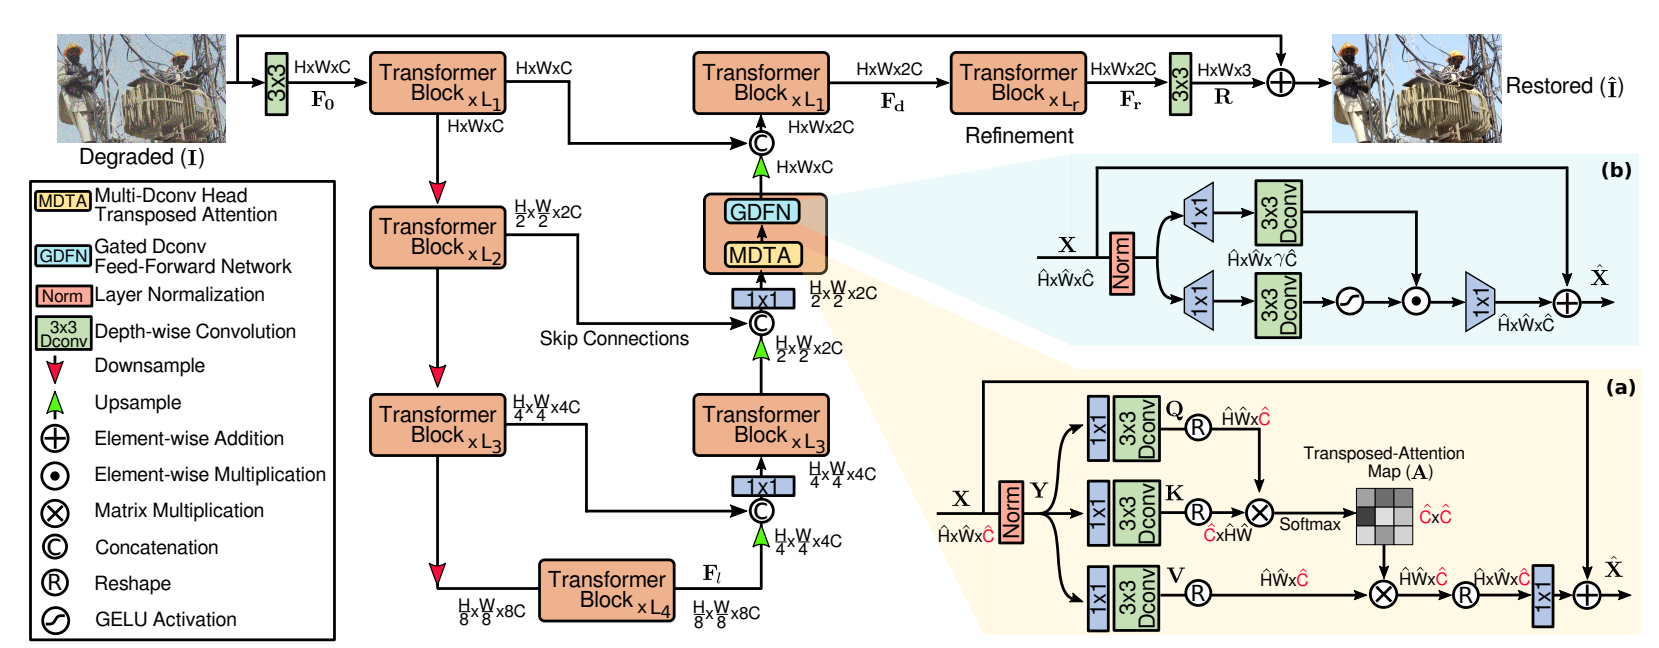
\includegraphics[scale=0.29]{figures/Architecture_of_Restormer.png}
\caption{Restomerのアーキテクチャ全体図. 文献\cite{Restormer}より引用. (C) 2022 IEEE/CVF \label{fig:Restomer_overall}}
\end{figure}

 
\chapter{提案手法}
既存手法であるGTCNNにおいて, コンテクスト抽出を担うGTLはU-Netをベースに設計されている. 本論文ではGTLの各層にCNN以上にコンテクスト抽出性能の優れたTransformerを組み込んだ手法, SAGTCNN (Self-Attention GTCNN) を提案する. Transformerを挿入する場所を変更したいくつかのバージョンを提案し, それらの性能を比較する. 実験を通して, Transformerのヘッドの数は1としている. 提案手法はGTLを変更した以外は従来のGTCNNのアーキテクチャを踏襲している. またパラメータサイズの比較は表\ref{tab:p_size}にて示している.

\section{SAGTCNN-S4}
SAGTCNN-S4は図\ref{fig:GTL_S4}のような構造になっている. 青い枠の部分が従来手法に変更を加えたところである. 従来手法では全ての層がCNN Blockで形成されていたがSAGTCNN-S4では4段目をSA Blockに変更しているところに特徴がある. さらに, プーリングよるダウンサンプリングを畳み込みで行うようにし, バイリニアでのアップサンプリングを畳み込みで行うように変更した. SA Blockは畳み込みを2度行うD-conv層とAttention層の2層からなっている. Transformerは画像のスケールが大きくなるほど計算量が増大するため, スケールの小さい4段目でTransformerを用いることで計算量の増大を防いでいる. 

\begin{figure}[htbp]
\centering
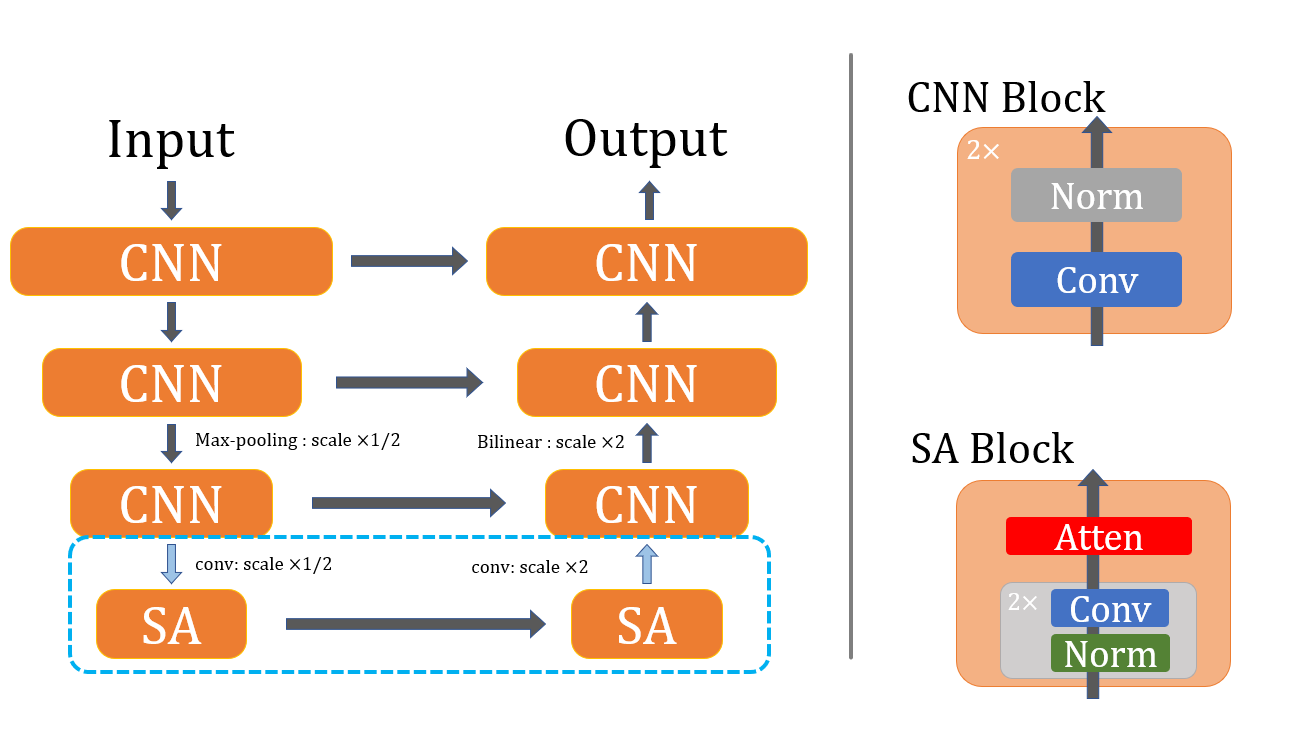
\includegraphics[scale=0.4]{figures/GTL_TS4.png}
\caption{SAGTCNN-S4のGTLのアーキテクチャ \label{fig:GTL_S4}}
\end{figure}

\newpage
\section{SAGTCNN-M}
SAGTCNN-Mでは本来なんの処理もなされていなかったミドル層にTransformerを追加した. アーキテクチャは図\ref{fig:GTL_M}の通りである. ミドル層は他の層と比べてスケールが最も小さくTransformerの処理も最も軽いため, 効率的にノイズ除去性能の向上を行える可能性があり実験を行った.

\begin{figure}[htbp]
\centering
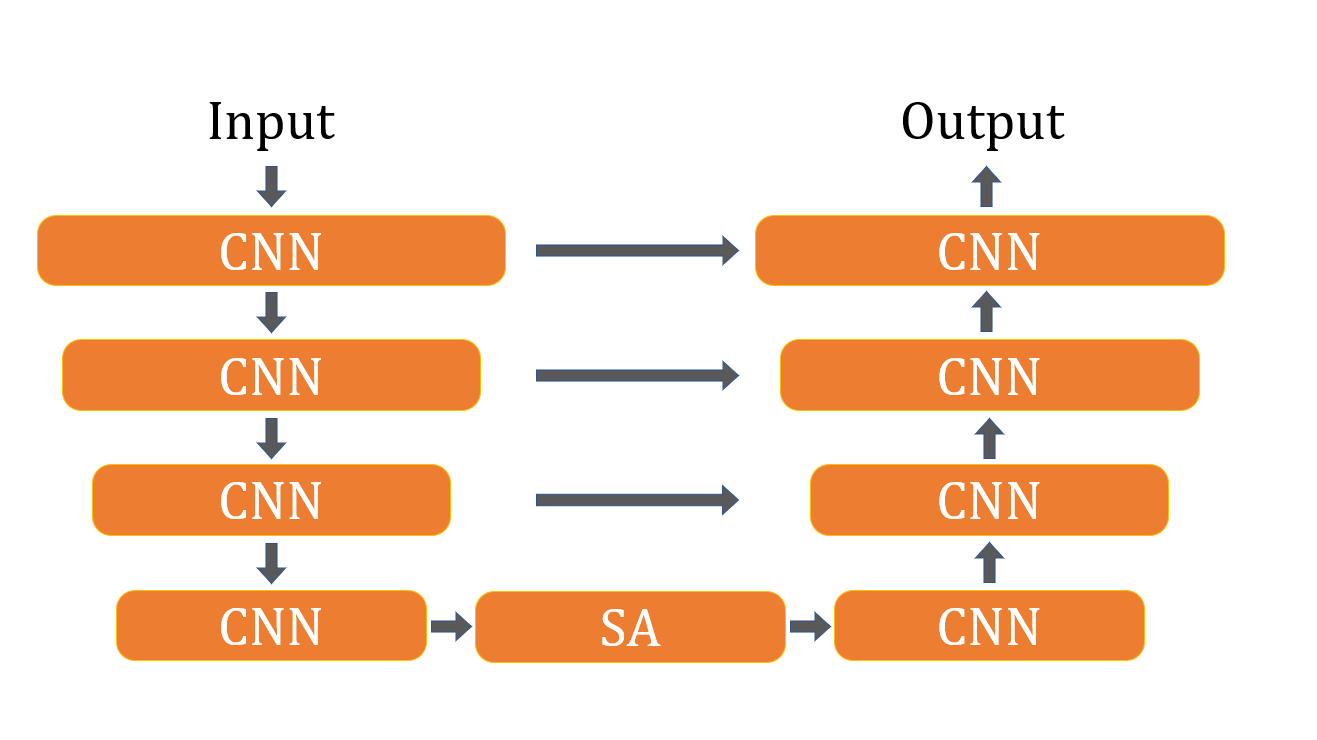
\includegraphics[scale=0.3]{figures/GTL_M.png}
\caption{SAGTCNN-MのGTLのアーキテクチャ \label{fig:GTL_M}}
\end{figure}

\section{SAGTCNN-S4M}
SAGTCNN-S4およびSAGTCNN-Mを合わせた手法で, Transformerを4段目とミドル層に挿入した. 計算量およびパラメータサイズは他の手法より大きくなる. 

\begin{table}[htbp]
\centering
\caption{パラメータサイズの比較 \label{tab:p_size}}
 \begin{tabular}{|c|c|c|c|}
 \hline
 GTCNN & SAGTCNN-S4 & SAGTCNN-M & SAGTCNN-S4M \\ \hline \hline 
   $\mathbf{851k}$ & 996k & 1,016k & 1,161k \\ \hline
 \end{tabular}
\end{table}
\chapter{実験}
提案手法の有効性を調べるため, 既存手法と提案手法のノイズ除去性能を比べた. その際, 生成ノイズを加算したグレースケール画像に対するノイズ除去性能を比較した.

\section{実験設定}
概ねGTCNNの設定に従って実験を行う\cite{GTCNN}.

\subsection{ネットワーク構成}
既存手法GTCNNのCBR層の数を1つに固定した. 提案手法である自己注意機構を追加したGTCNN(Self-Attention GTCNN: 以後SAGTCNN)はGTLの4層目のCNNを自己注意に置き換えたSAGTCNN-S4, ミドル層に自己注意を追加したSAGTCNN-M, そのどちらの変更を加えたSAGTCNN-S4Mの3種類のパターンで比較を行った. GTCNNおよびSAGTCNNのGTLは共に同じ段数($S=4$)で構成した.

\subsection{学習設定}
データセットにはDIV2Kを用いる. DIV2Kの全画像から$192 \times 192$画素のパッチをストライド192画素で切り出したものを学習画像とする. 学習のエポック数は600とする.

\subsection{評価手法}
既存手法と同様に, ノイズ除去評価手法において一般的に使われるガウシアンノイズを原画像に加算した画像(生成ノイズ画像)から原画像を推定する. ノイズ除去結果の評価はPSNRを用いる. 原画像にはSet12, BSD68, Urban100のデータセットを使用した. 従来手法であるGTCNNの評価値は, 論文に記載されている値を引用した.

\section{実験結果}
表\ref{tab:sigma50}に示すように$\sigma=50$での性能比較の結果, 今回SAGTCNNで試したどのパターンにおいても既存手法の性能を上回ることはなかった. SAGTCNNの中で最も性能の高いSAGTCNN-S4とGTCNNを$\sigma$の値を30, 50, 70と変更して比較しても, 表\ref{tab:sigmaxx}の通り性能の向上は見られなかった. SAGTCNN-MはUrban100のデータセットにて他の手法と比べて性能が特に悪い. 出力画像の一枚を比べると他の手法より画像が劣化していることが図\ref{fig:Outputs}から分かる. 

\begin{table}[htbp]
\centering
\caption{生成ノイズ$\sigma=50$におけるGTCNNとSAGTCNNの性能比較 \label{tab:sigma50}}
 \begin{tabular}{|l||c|c|c|}
 \hline
 手法 & Set12 & BSD68 & Urban100 \\ \hline \hline
 GTCNN         & $\bm{27.56}$ & $\bm{26.46}$ & $\bm{26.97}$ \\ \hline
 SAGTCNN-S4    & 27.55 & 26.43 & 26.95 \\ \hline
 SAGTCNN-M     & 27.55 & 26.29 & 23.48 \\ \hline
 SAGTCNN-S4M   & 27.47 & 26.38 & 26.84 \\ \hline
 \end{tabular}
\end{table}


\begin{table}[htbp]
\centering
\caption{生成ノイズの$\sigma$の値を変更した時のGTCNNとSAGTCNNの性能比較 \label{tab:sigmaxx}}
\setlength\tabcolsep{1.5pt}
 \begin{tabular}{|l|c|c|c|c|c|c|c|c|c|}
\hline
\multirow{2}{*}{手法} &  \multicolumn{3}{c|}{Set12} &  \multicolumn{3}{c|}{BSD68} &  \multicolumn{3}{c|}{Urban100}   \\
\cline{2-10}
 & 30 & 50 & 70  & 30 & 50 & 70  & 30 & 50 & 70 \\
\hline \hline
GTCNN & 29.80 
            & $\bm{27.56}$ 
                & $\bm{26.08}$ 
                    
                    & $\bm{28.53}$ 
                        & $\bm{26.46}$ 
                            & $\bm{25.21}$ 
                            
                                & 29.43 
                                    & $\bm{26.97}$ 
                                        & $\bm{25.36}$ \\ \hline
SAGTCNN-S4    & $\bm{29.81}$ 
                &  27.55 
                    & 26.07 
                    
                    & 28.52 
                        & 26.43 
                            & 25.19 
                                
                                & $\bm{29.46}$ 
                                    & 26.95 
                                        & 25.34 \\ \hline
 \end{tabular}
\end{table}

\begin{table}[htbp]
\centering
\caption{SAGTCNNの学習画像を増加させた際の変化:NormalはDIV2Kのみ. IncreaseはDIV2K+SSID \label{tab:manyImage}}
 \begin{tabular}{|l||c|c|c|}
 \hline
 手法 & Set12 & BSD68 & Urban100 \\ \hline \hline
 SAGTCNN-S4 (Normal)        & 27.55 & 26.43 & 26.95 \\ \hline
 SAGTCNN-S4 (Increase)     & 27.52 & 26.43 & 26.90 \\ \hline
 \end{tabular}
\end{table}



\begin{figure}[htbp]
\centering
\includegraphics[scale=1.0]{figures/Outputs.png}
\caption{出力画像比較 \label{fig:Outputs}}
\end{figure}

\newpage
\section{考察}
実験ではGTCNNに対しSAGTCNNは生成ノイズ$\sigma = 30$の場合においてノイズ除去性能をわずかに上回った. ものの, 明確な優位性を示すことはできなかった. 過学習の懸念から学習画像枚数を増やしてみたものの, 表\ref{tab:manyImage}の通り, 性能が向上することはなかった. ノイズ除去性能の向上が見られなかった理由はいくつか考えられる. まず一般的に自己注意を用いる手法では大規模なデータセットを用いており, 今回の実験で使用した学習用のデータセットでは学習画像枚数が少ない可能性が考えられる. また自己注意は広域のコンテクストを捉えることを得意とするが, 今回GTLの4段目という画像サイズの小さい領域でしか自己注意を用いておらず, 本来の性能が活かせなかったことが考えられる. 最後に画像に自己注意を用いる際にViTなどで行われている位置埋め込みを本実験では行っていないため, コンテクストの抽出が上手く行えなかった可能性が考えられる. 



\chapter{結論}
本論文では, GTCNNのコンテクスト抽出を行うGTLに自己注意機構を組み込んだ手法, SAGTCNNを提案した. 自己注意機構を挿入する場所を変更したSAGTCNN-S4, SAGTCNN-M, SAGTCNN-S4Mの3種類のパターンで実験を行った. 実験ではGTCNNに対しSAGTCNNはいくつかのケースでわずかに上回る性能を示した一方で, 明確な優位性を示すことはできなかった. ノイズ除去性能の向上があまり見られなかった理由はいくつか考察できる. まず一般的に自己注意を用いる手法では大規模なデータセットを用いており, 今回の実験で使用した学習用のデータセットでは学習画像枚数が少ない可能性が考えられる. また, 自己注意は広域のコンテクストを捉えることを得意とするが, 今回GTLの4段目という画像サイズの小さい領域でしか自己注意を用いておらず, 本来の性能が活かせなかったことが考えられる. 最後に画像に自己注意を用いる際にViTなどで行われている位置埋め込みを本実験では行っていないため, コンテクストの抽出が上手く行えなかった可能性が考えられる. \\
 今後の課題としては, 位置埋め込みの実装やリアルノイズでの性能比較, 自己注意をGTLの上層にて使用した際の有効性の検討などが挙げられる. 


%%%%%%%%%%%%%%%%%%%%%%%%%%%%%%%%%%%%%%%%%%%%%%%%%%%%%%%%%%%%%%%%

\chapter*{謝辞}
\addcontentsline{toc}{chapter}{謝辞}
本研究を進めるにあたり, 様々な助言および御指導を賜った宮田高道教授に心より感謝いたします. またGTCNNのコードをお借りした今井海斗氏にも深く感謝いたします. 研究室の同輩や先輩の方々にも助けて頂きました感謝いたします.

\nocite{*}
\cleardoublepage
\pagestyle{plain}

\bibliography{ref}


%図の一覧を出力する場合
%\listoffigures

%表の一覧を出力する場合
%\listoftables

\end{document}
